% !TEX root = ../main.tex

\clearpage
% Source PDF page 30.
\section{第九章\quad 奶蛙进校园——高校奶蛙活动概述}

本章将提及一些高校奶蛙活动，不分先后。由于编者精力极度有限，如果读者学校的奶蛙活动未被提及，也请谅解。奶蛙无高低，快乐最重要嘛。

\subsection{一、各自为战的高校奶蛙}

\subsubsection{（1）哈尔滨工业大学}

2026 年 6 月，在哈尔滨工业大学深圳校区的 2026 年毕业典礼暨学位授予仪式上出现了第一个广为人知的奶蛙立牌。哈工大奶蛙立牌的强势出镜破圈，标志着各大学正式进入了奶蛙立牌争先赶超、军备竞赛的阶段的阶段。~(见\figref{fig:09-1})

% !TEX root = ../../main.tex
\begin{figure}[H]
  \centering
  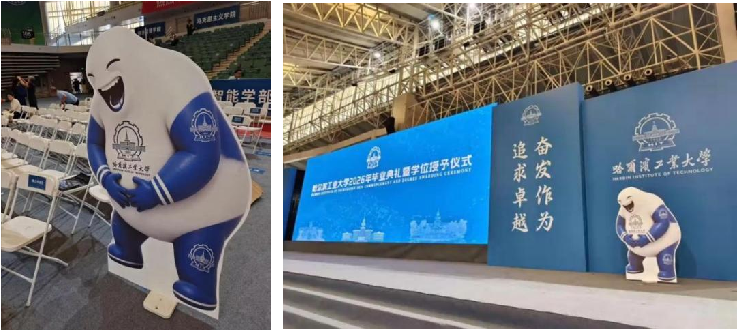
\includegraphics[width=301.14bp,height=0.76\textheight,keepaspectratio]{figures/chapter09/figure09_1.pdf}
  \renewcommand{\thefigure}{9.1}
  \caption{哈尔滨工业大学 2026 年毕业典礼暨学位授予仪式上的奶蛙立牌}
  \label{fig:09-1}
\end{figure}


\subsubsection{（2）武汉大学}

据当前可查询到的信息资料，武汉大学是最早发起流动奶蛙活动的高校（2026/9/12 晚 5 点前后），并且在奶蛙大流动前便拥有千人级别的奶龙群。~(见\figref{fig:09-2})

% !TEX root = ../../main.tex
\begin{figure}[H]
  \centering
  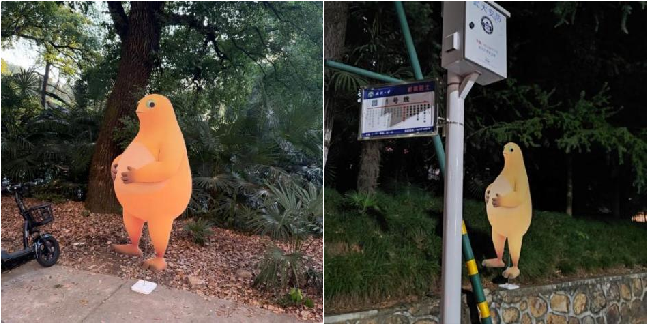
\includegraphics[width=263.19bp,height=0.76\textheight,keepaspectratio]{figures/chapter09/figure09_2.pdf}
  \renewcommand{\thefigure}{9.2}
  \caption{武汉大学的奶蛙立牌的出生点（左）和奶狗气球车（右）}
  \label{fig:09-2}
\end{figure}


在流动奶蛙活动中，同学们可以把奶蛙带到学校各个角落，在任意一处地方偶遇惊喜。这一行为与\textbf{四川农业大学的“搬牛”活动}不谋而合。武大作为流动奶蛙的先驱，为流动奶蛙这一活动打下了范式，揭开了奶蛙立牌时代的序幕。距离较近的华中师范大学与中南财经政法大学紧随其后加入。

\subsubsection{（3）上海交通大学}

上海交通大学集思广益（迫真），紧随武大脚步发起了新一次的大型流动奶蛙活动，并且取得了前所未有的破圈效果。这标志着奶蛙立牌的全面爆火，为奶蛙立牌全面进入校园和奶蛙时代的开启打下了坚实基础。

下为上交最初的流动奶蛙。到本书成书为止仍在使用。~(见\figref{fig:09-3})

\clearpage
% Source PDF page 31.
% !TEX root = ../../main.tex
\begin{figure}[H]
  \centering
  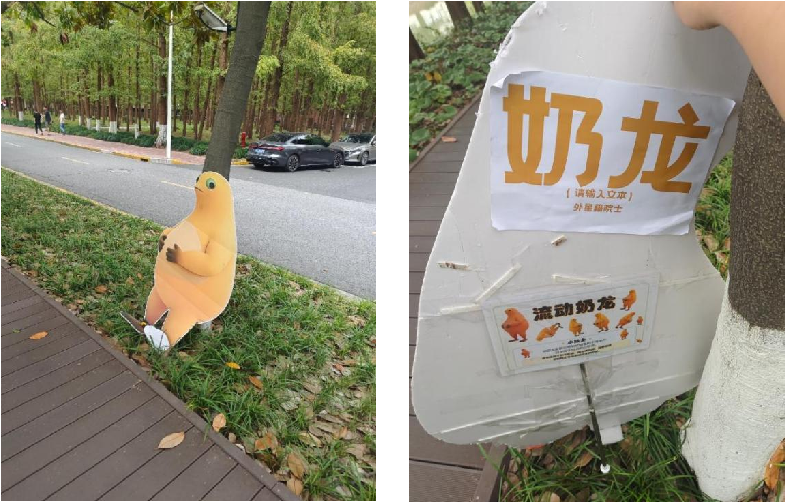
\includegraphics[width=320.62bp,height=0.76\textheight,keepaspectratio]{figures/chapter09/figure09_3.pdf}
  \renewcommand{\thefigure}{9.3}
  \caption{上海交通大学的流动奶蛙立牌}
  \label{fig:09-3}
\end{figure}


\subsubsection{（4）中国海洋大学}

中国海洋大学最为出圈的无疑是“奶 OUC”的四奶蛙立牌。这是第一个广为人知的复数奶蛙立牌，为其他学校提制作更多花样奶蛙立牌打开了思路。~(见\figref{fig:09-4}, \figref{fig:09-5})

% !TEX root = ../../main.tex
\begin{figure}[H]
  \centering
  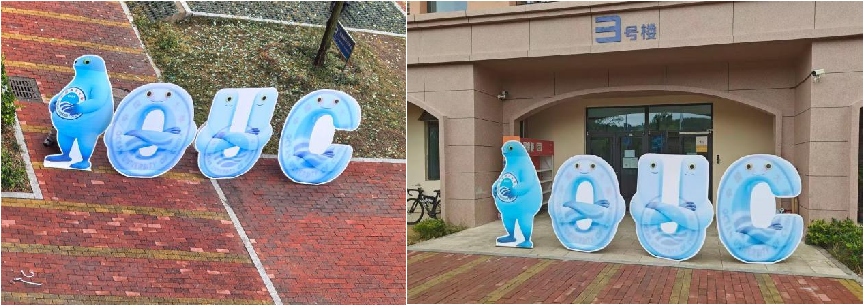
\includegraphics[width=352.34bp,height=0.76\textheight,keepaspectratio]{figures/chapter09/figure09_4.pdf}
  \renewcommand{\thefigure}{9.4}
  \caption{海大的“奶 OUC”四奶蛙立牌}
  \label{fig:09-4}
\end{figure}


% !TEX root = ../../main.tex
\begin{figure}[H]
  \centering
  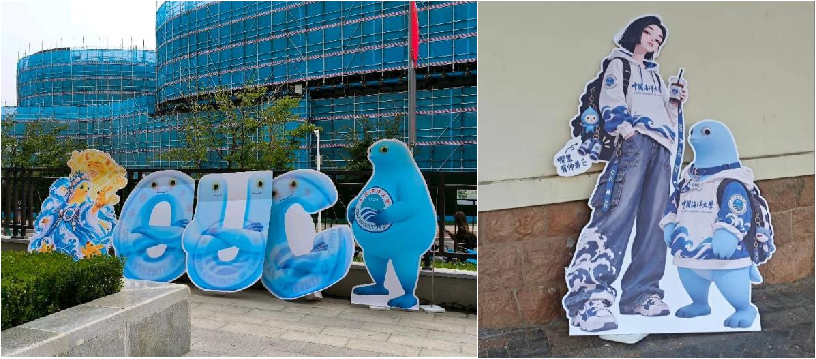
\includegraphics[width=332.96bp,height=0.76\textheight,keepaspectratio]{figures/chapter09/figure09_5.pdf}
  \renewcommand{\thefigure}{9.5}
  \caption{海大奶蛙立牌组完全体形态（左）和绝代双糖（右）}
  \label{fig:09-5}
\end{figure}


\clearpage
% Source PDF page 32.
海大更有院级奶牌，这一思路启发了各高校奶牌的百花齐放。~(见\figref{fig:09-6})

% !TEX root = ../../main.tex
\begin{figure}[H]
  \centering
  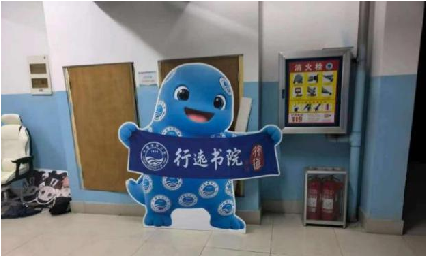
\includegraphics[width=174.05bp,height=0.76\textheight,keepaspectratio]{figures/chapter09/figure09_6.pdf}
  \renewcommand{\thefigure}{9.6}
  \caption{海大行远书院的院级奶龙立牌}
  \label{fig:09-6}
\end{figure}


\subsubsection{（5）浙江大学}

浙江大学在某地的招生宣传立牌中，出现了浙大奶蛙的形象。由于时间无法确定，编者决定将其放在这里。~(见\figref{fig:09-7})

% !TEX root = ../../main.tex
\begin{figure}[H]
  \centering
  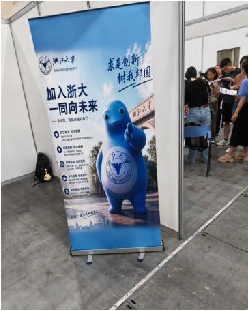
\includegraphics[width=101.63bp,height=0.76\textheight,keepaspectratio]{figures/chapter09/figure09_7.pdf}
  \renewcommand{\thefigure}{9.7}
  \caption{浙大带有奶蛙的招生宣传立牌}
  \label{fig:09-7}
\end{figure}


\subsubsection{（6）北京航空航天大学}

北京航空航天大学的奶龙同好会成立于 2026 年 6 月 24 日。最开始的成立目标是为了让原飞梦社的抽象老登们有个神圣的水群，但是由于奶蛙前所未有的强横热度，人数激增，在 2026 年 8 月初便突破 100 人，在 26 级新生入学后更涌入大量新鲜血液，于 2026 年 9 月 30 日突破 200 人，成为飞梦之后北航校园文化新的中坚力量之一。~(见\figref{fig:09-8})

% !TEX root = ../../main.tex
\begin{figure}[H]
  \centering
  
\includegraphics[width=272.68bp,height=0.76\textheight,keepaspectratio]{figures/chapter09/figure09_8.pdf}
  \renewcommand{\thefigure}{9.8}
  \caption{北航奶龙同好会 100 人贺图（左）及 200 人贺图（右）}
  \label{fig:09-8}
\end{figure}


\clearpage
% Source PDF page 33.
下为 BUAAer 制作的一些北航奶蛙表情包。~(见\figref{fig:09-9})

% !TEX root = ../../main.tex
\begin{figure}[H]
  \centering
  
\includegraphics[width=260.44bp,height=0.76\textheight,keepaspectratio]{figures/chapter09/figure09_9.pdf}
  \renewcommand{\thefigure}{9.9}
  \caption{北航数分奶蛙（左） 捧着航概的奶蛙（中） 校徽奶蛙（右）}
  \label{fig:09-9}
\end{figure}


2026 年 9 月 28 日，一个神秘人在北航学院路校区绿园投放了流动奶蛙立牌。~(见\figref{fig:09-10})

% !TEX root = ../../main.tex
\begin{figure}[H]
  \centering
  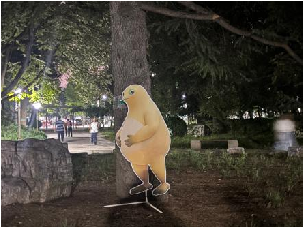
\includegraphics[width=123.86bp,height=0.76\textheight,keepaspectratio]{figures/chapter09/figure09_10.pdf}
  \renewcommand{\thefigure}{9.10}
  \caption{北航学院路校区绿园奶蛙立牌}
  \label{fig:09-10}
\end{figure}


旁边随后还出现了丰川祥子的立牌。学院路的学生们纷纷与之开心合影。~(见\figref{fig:09-11})

% !TEX root = ../../main.tex
\begin{figure}[H]
  \centering
  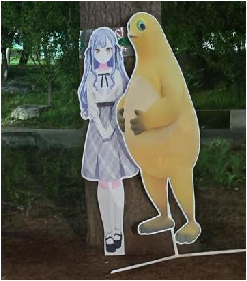
\includegraphics[width=100.81bp,height=0.76\textheight,keepaspectratio]{figures/chapter09/figure09_11.pdf}
  \renewcommand{\thefigure}{9.11}
  \caption{北航学院路校区绿园奶蛙立牌和祥子立牌}
  \label{fig:09-11}
\end{figure}


当晚，奶蛙立牌和祥子立牌被保安发现，立牌被带走，存活约 9 小时。BUAA奶龙同好会对此深表遗憾。下为大家自愿为奶蛙立牌刷屏的一段赞诗：

\begin{center}
\itshape
\fontsize{10.5}{13}\selectfont
我的肉化作黄桃罐头\\
我的血化为蜂蜜\\
我是从天上降下的生活的食粮\\
谁若吃了这食粮\\
必要大笑直到永远\\
我所要赐的食粮\\
就是我的肉\\
为使世界获得笑容。
\end{center}

正因为奶家人的热情，奶蛙在 BUAA 的故事绝不会到此为止。2026 年 10 月2 日，北航沙河校区 TD 线旁出现奶蛙立牌，但被保安迅速逮捕。2026 年 10 月 8日，北航杭州校区出现奶蛙立牌。至此，北航实现了全部校区的奶蛙立牌覆盖。~(见\figref{fig:09-12})

\clearpage
% Source PDF page 34.
% !TEX root = ../../main.tex
\begin{figure}[H]
  \centering
  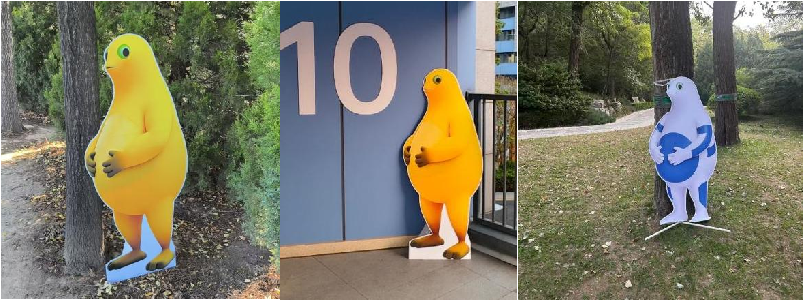
\includegraphics[width=328.17bp,height=0.76\textheight,keepaspectratio]{figures/chapter09/figure09_12.pdf}
  \renewcommand{\thefigure}{9.12}
  \caption{北航沙航奶蛙立牌（左）、杭航奶蛙立牌（中）和学航二代奶蛙立牌（右）}
  \label{fig:09-12}
\end{figure}


2026 年 10 月 9 日，北航沙河校区在 SH2 地下二层的室内完成了全世界首只飞行奶蛙的飞行实现，并取得了完全成功，开创出了北航作为一所航空航天院校的独有奶蛙之路。~(见\figref{fig:09-13})

（飞行奶蛙 B 站视频号：BV1gnps6LEF3）

% !TEX root = ../../main.tex
\begin{figure}[H]
  \centering
  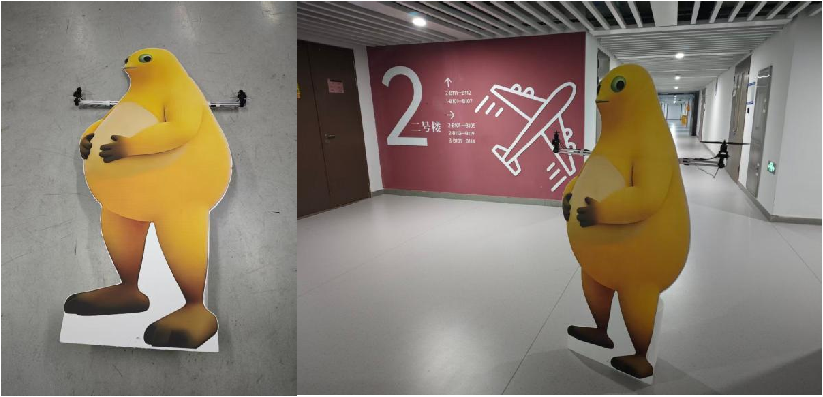
\includegraphics[width=335.92bp,height=0.76\textheight,keepaspectratio]{figures/chapter09/figure09_13.pdf}
  \renewcommand{\thefigure}{9.13}
  \caption{北航沙河校区首只飞行奶蛙试飞现场}
  \label{fig:09-13}
\end{figure}


2026 年 10 月 16 日，BUAA 奶龙同好会出品了奶科学与大笑工程学院培养方案，并绘制了徽标，为可能的奶教学事业画好了蓝图。~(见\figref{fig:09-14})

% !TEX root = ../../main.tex
\begin{figure}[H]
  \centering
  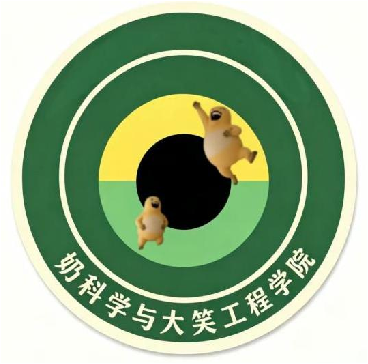
\includegraphics[width=150.28bp,height=0.76\textheight,keepaspectratio]{figures/chapter09/figure09_14.pdf}
  \renewcommand{\thefigure}{9.14}
  \caption{北航奶龙同好会的奶科学与大笑工程学院标志}
  \label{fig:09-14}
\end{figure}


\clearpage
% Source PDF page 35.
\subsubsection{（7）广东海洋大学}

作为最早一批的奶蛙立牌开拓者，广海的奶蛙立牌在网上同样引发了巨大的反响。谁不想在军训期间被一只奶蛙陪着呢？~(见\figref{fig:09-15})

% !TEX root = ../../main.tex
\begin{figure}[H]
  \centering
  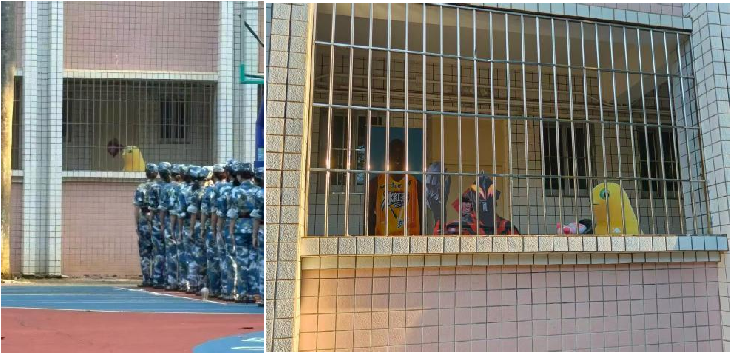
\includegraphics[width=298.38bp,height=0.76\textheight,keepaspectratio]{figures/chapter09/figure09_15.pdf}
  \renewcommand{\thefigure}{9.15}
  \caption{广海的军训奶蛙立牌（左）和“一门四至尊”（右）}
  \label{fig:09-15}
\end{figure}


\subsubsection[（8）南方科技大学]{（8）南方科技大学~(见\figref{fig:09-16})}

% !TEX root = ../../main.tex
\begin{figure}[H]
  \centering
  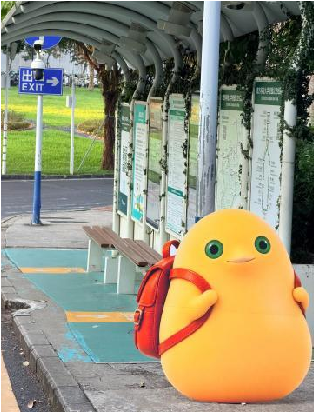
\includegraphics[width=128.45bp,height=0.76\textheight,keepaspectratio]{figures/chapter09/figure09_16.pdf}
  \renewcommand{\thefigure}{9.16}
  \caption{南科大公交站点的奶蛋立牌}
  \label{fig:09-16}
\end{figure}


\subsubsection[（9）山东大学]{（9）山东大学~(见\figref{fig:09-17})}

% !TEX root = ../../main.tex
\begin{figure}[H]
  \centering
  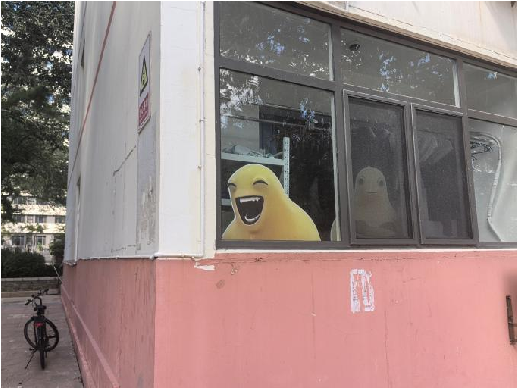
\includegraphics[width=211.17bp,height=0.76\textheight,keepaspectratio]{figures/chapter09/figure09_17.pdf}
  \renewcommand{\thefigure}{9.17}
  \caption{山大的大笑奶蛙立牌和抱胸奶蛙立牌}
  \label{fig:09-17}
\end{figure}


\clearpage
% Source PDF page 36.
\subsubsection{（10）华中科技大学}~(见\figref{fig:09-18})

% !TEX root = ../../main.tex
\begin{figure}[H]
  \centering
  
\includegraphics[width=117.74bp,height=0.76\textheight,keepaspectratio]{figures/chapter09/figure09_18.pdf}
  \renewcommand{\thefigure}{9.18}
  \caption{华科的左右护法大笑奶蛙立牌}
  \label{fig:09-18}
\end{figure}


2026 年 10 月 10 日，由于华中科技大学奶蛙同好会高层犯下了严重错误，大量华科奶蛙同好会成员对华科奶龙同好会进行爆破，使双方爆发激烈冲突，最终直接导致首届华科奶蛙同好会的解散。对奶龙奶蛙的错误思想使华科的奶龙奶蛙运动受到重创，值得各高校的奶民深思。

\subsubsection[（11）复旦大学]{（11）复旦大学~(见\figref{fig:09-19}, \figref{fig:09-20})}

% !TEX root = ../../main.tex
\begin{figure}[H]
  \centering
  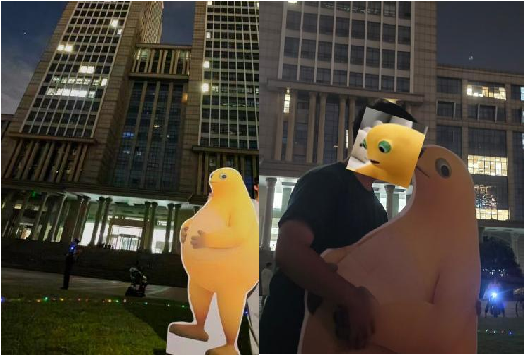
\includegraphics[width=214.13bp,height=0.76\textheight,keepaspectratio]{figures/chapter09/figure09_19.pdf}
  \renewcommand{\thefigure}{9.19}
  \caption{复旦学子与奶蛙立牌激情合照}
  \label{fig:09-19}
\end{figure}


% !TEX root = ../../main.tex
\begin{figure}[H]
  \centering
  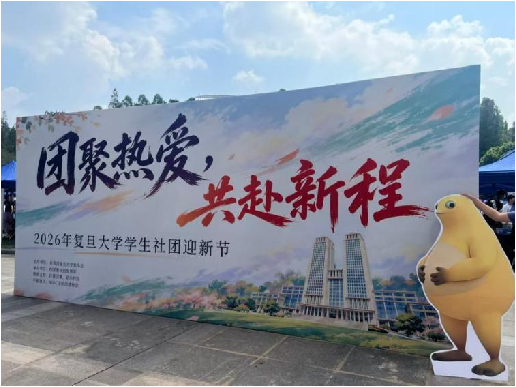
\includegraphics[width=210.56bp,height=0.76\textheight,keepaspectratio]{figures/chapter09/figure09_20.pdf}
  \renewcommand{\thefigure}{9.20}
  \caption{进军复旦百团活动的奶蛙立牌}
  \label{fig:09-20}
\end{figure}


\clearpage
% Source PDF page 37.
\subsubsection{（12）清华大学}

清华变“清蛙”，清华门的沦陷，昭示着奶蛙的大手已经无处不在。~(见\figref{fig:09-21}, \figref{fig:09-22})

% !TEX root = ../../main.tex
\begin{figure}[H]
  \centering
  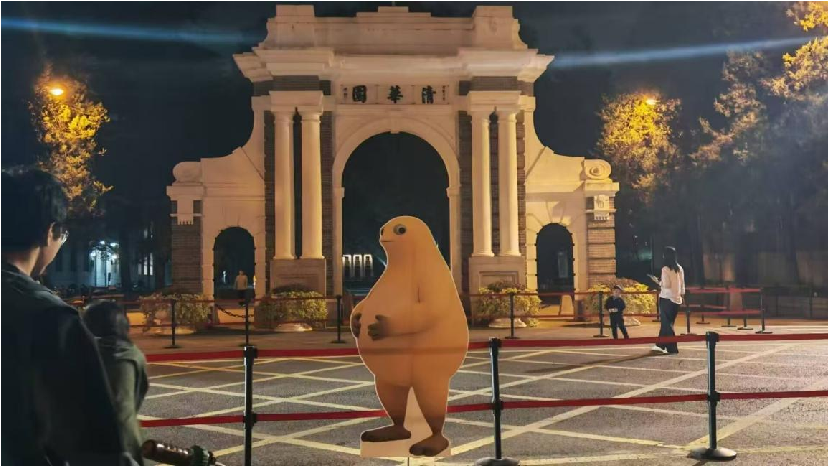
\includegraphics[width=338.27bp,height=0.76\textheight,keepaspectratio]{figures/chapter09/figure09_21.pdf}
  \renewcommand{\thefigure}{9.21}
  \caption{奶蛙占领清华门}
  \label{fig:09-21}
\end{figure}


% !TEX root = ../../main.tex
\begin{figure}[H]
  \centering
  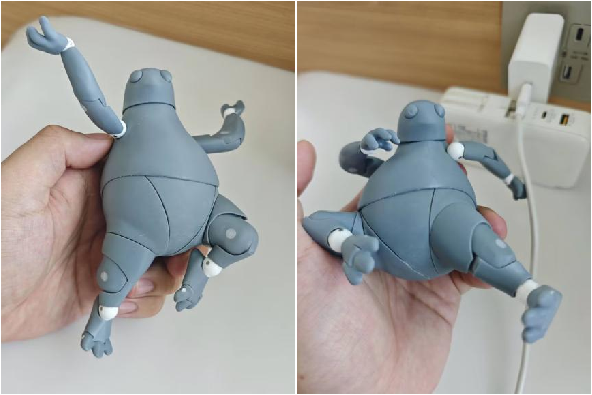
\includegraphics[width=241.47bp,height=0.76\textheight,keepaspectratio]{figures/chapter09/figure09_22.pdf}
  \renewcommand{\thefigure}{9.22}
  \caption{清华学生制作的高自由度可动奶蛙手办}
  \label{fig:09-22}
\end{figure}


\subsubsection[（13）北京理工大学]{（13）北京理工大学~(见\figref{fig:09-23}, \figref{fig:09-24}, \figref{fig:09-25})}

% !TEX root = ../../main.tex
\begin{figure}[H]
  \centering
  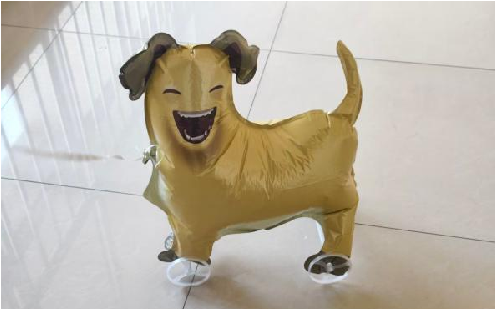
\includegraphics[width=202.5bp,height=0.76\textheight,keepaspectratio]{figures/chapter09/figure09_23.pdf}
  \renewcommand{\thefigure}{9.23}
  \caption{北理的奶狗气球车}
  \label{fig:09-23}
\end{figure}


\clearpage
% Source PDF page 38.
% !TEX root = ../../main.tex
\begin{figure}[H]
  \centering
  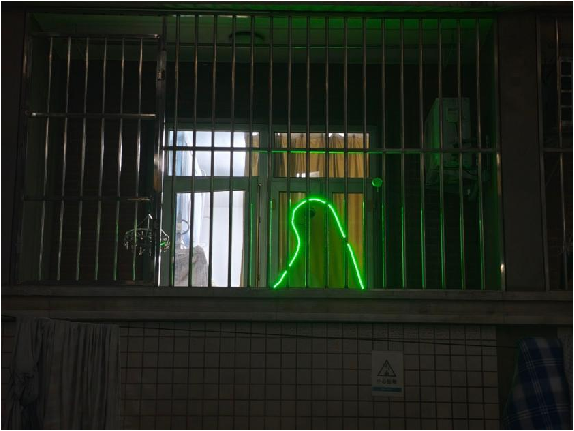
\includegraphics[width=234.12bp,height=0.76\textheight,keepaspectratio]{figures/chapter09/figure09_24.pdf}
  \renewcommand{\thefigure}{9.24}
  \caption{北理的夜光奶蛙}
  \label{fig:09-24}
\end{figure}


% !TEX root = ../../main.tex
\begin{figure}[H]
  \centering
  
\includegraphics[width=128.45bp,height=0.76\textheight,keepaspectratio]{figures/chapter09/figure09_25.pdf}
  \renewcommand{\thefigure}{9.25}
  \caption{北理的奶味校徽“北蛙理工大学”}
  \label{fig:09-25}
\end{figure}


\subsubsection[（14）电子科技大学]{（14）电子科技大学~(见\figref{fig:09-26})}

% !TEX root = ../../main.tex
\begin{figure}[H]
  \centering
  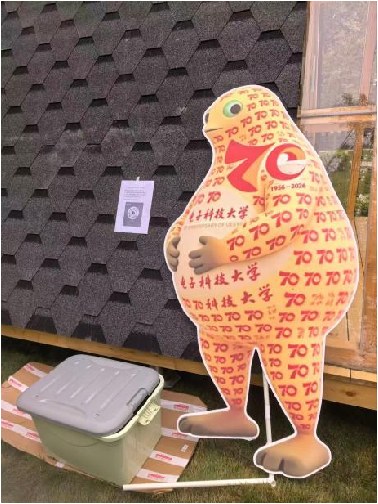
\includegraphics[width=154.36bp,height=0.76\textheight,keepaspectratio]{figures/chapter09/figure09_26.pdf}
  \renewcommand{\thefigure}{9.26}
  \caption{电科的花龙立牌}
  \label{fig:09-26}
\end{figure}


\clearpage
% Source PDF page 39.
\subsubsection{（15）辽宁工程技术大学}

% !TEX root = ../../main.tex
\begin{figure}[H]
  \centering
  
\includegraphics[width=281.15bp,height=0.76\textheight,keepaspectratio]{figures/chapter09/figure09_27.pdf}
  \renewcommand{\thefigure}{9.27}
  \caption{辽工大的原味校徽（左）和奶味校徽（右）}
  \label{fig:09-27}
\end{figure}


辽工大作为校徽上自带两个奶蛙形状的大学，在网上很早便有了名气，一直被人们津津乐道。~(见\figref{fig:09-27})

\subsubsection[（16）中国科学院大学]{（16）中国科学院大学~(见\figref{fig:09-28})}

% !TEX root = ../../main.tex
\begin{figure}[H]
  \centering
  
\includegraphics[width=259.11bp,height=0.76\textheight,keepaspectratio]{figures/chapter09/figure09_28.pdf}
  \renewcommand{\thefigure}{9.28}
  \caption{国科的奶味徽标（左）和国科大的奶龙科学院大学网址（右）}
  \label{fig:09-28}
\end{figure}


\subsubsection[（17）同济大学]{（17）同济大学~(见\figref{fig:09-29})}

% !TEX root = ../../main.tex
\begin{figure}[H]
  \centering
  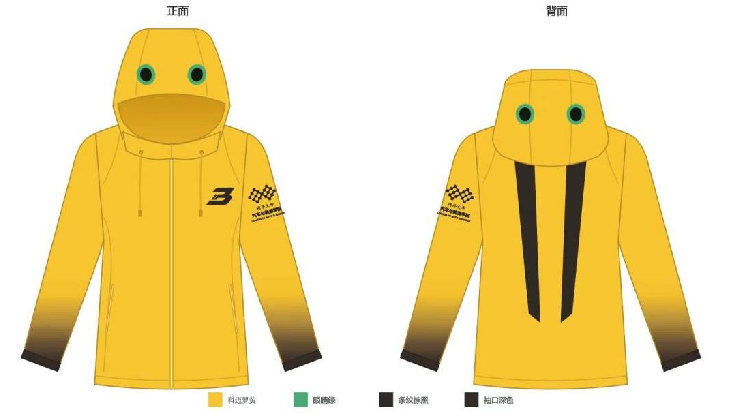
\includegraphics[width=297.98bp,height=0.76\textheight,keepaspectratio]{figures/chapter09/figure09_29.pdf}
  \renewcommand{\thefigure}{9.29}
  \caption{同济材料学院的奶味队服设计概念图}
  \label{fig:09-29}
\end{figure}


\clearpage
% Source PDF page 40.
\subsubsection{（18）北京大学}

% !TEX root = ../../main.tex
\begin{figure}[H]
  \centering
  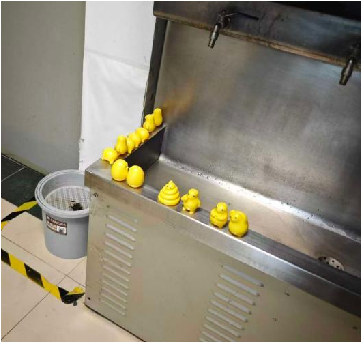
\includegraphics[width=147.83bp,height=0.76\textheight,keepaspectratio]{figures/chapter09/figure09_30.pdf}
  \renewcommand{\thefigure}{9.30}
  \caption{北大放满奶味手办的饮水机}
  \label{fig:09-30}
\end{figure}


值得惋惜的是，同为 Top2 的 PKU 没有像 THU 一样开放，而是对奶蛙进行了严密封锁。即使在宿舍内部张贴奶蛙相关贴画、摆放立牌也会被检查没收，在校内论坛发奶蛙/奶龙字样大概率就会被封禁。~(见\figref{fig:09-30})

\subsubsection[（19）北京师范大学]{（19）北京师范大学~(见\figref{fig:09-31})}

% !TEX root = ../../main.tex
\begin{figure}[H]
  \centering
  
\includegraphics[width=250.04bp,height=0.76\textheight,keepaspectratio]{figures/chapter09/figure09_31.pdf}
  \renewcommand{\thefigure}{9.31}
  \caption{从北师大浴室洗完澡的奶蛙}
  \label{fig:09-31}
\end{figure}


\subsubsection[（20）北京农学院]{（20）北京农学院~(见\figref{fig:09-32})}

% !TEX root = ../../main.tex
\begin{figure}[H]
  \centering
  
\includegraphics[width=112.34bp,height=0.76\textheight,keepaspectratio]{figures/chapter09/figure09_32.pdf}
  \renewcommand{\thefigure}{9.32}
  \caption{北农憨态可掬的奶蛙形象}
  \label{fig:09-32}
\end{figure}


\clearpage
% Source PDF page 41.
\subsubsection{（21）兰州大学}~(见\figref{fig:09-33})

% !TEX root = ../../main.tex
\begin{figure}[H]
  \centering
  
\includegraphics[width=144.98bp,height=0.76\textheight,keepaspectratio]{figures/chapter09/figure09_33.pdf}
  \renewcommand{\thefigure}{9.33}
  \caption{兰大的奶蛙立牌}
  \label{fig:09-33}
\end{figure}


\subsubsection[（22）东北师范大学]{（22）东北师范大学~(见\figref{fig:09-34})}

% !TEX root = ../../main.tex
\begin{figure}[H]
  \centering
  
\includegraphics[width=282.37bp,height=0.76\textheight,keepaspectratio]{figures/chapter09/figure09_34.pdf}
  \renewcommand{\thefigure}{9.34}
  \caption{东北师大的奶龙文化传播研究所牌}
  \label{fig:09-34}
\end{figure}


\subsubsection[（23）上海理工大学]{（23）上海理工大学~(见\figref{fig:09-35})}

% !TEX root = ../../main.tex
\begin{figure}[H]
  \centering
  
\includegraphics[width=228.62bp,height=0.76\textheight,keepaspectratio]{figures/chapter09/figure09_35.pdf}
  \renewcommand{\thefigure}{9.35}
  \caption{上海理工大学的 120 周年校庆奶蛙立牌}
  \label{fig:09-35}
\end{figure}


\clearpage
% Source PDF page 42.
\subsection{二、前所未有的高校线上奶蛙大热潮}

2026 年 10 月 9 日，为促进各高校之间抑制不住的奶蛙热情，各高校之前成立了众多跨高校奶蛙群，如“世界奶蛙联合组织”群（简称世蛙会）、“各高校奶龙联合会”、“高校奶龙同好会”等，并且在各个高校的奶龙同好群之间互相传播各自奶龙同好会的群号，使得各个高校的奶龙同好会达到了空前绝后的规模。~(见\figref{fig:09-36})

% !TEX root = ../../main.tex
\begin{figure}[H]
  \centering
  
\includegraphics[width=133.04bp,height=0.76\textheight,keepaspectratio]{figures/chapter09/figure09_36.pdf}
  \renewcommand{\thefigure}{9.36}
  \caption{“世蛙会”的吉祥物奶蛙}
  \label{fig:09-36}
\end{figure}


在这股前所未有的热潮下，奶蛙旗帜被确定下来。奶蛙旗帜为整体黄色、中心有一绿一黑同心圆的旗帜，形成奶蛙一只眼睛的图案。奶蛙旗帜没有必须的尺寸比例限制。~(见\figref{fig:09-37})

% !TEX root = ../../main.tex
\begin{figure}[H]
  \centering
  
\includegraphics[width=118.15bp,height=0.76\textheight,keepaspectratio]{figures/chapter09/figure09_37.pdf}
  \renewcommand{\thefigure}{9.37}
  \caption{方形奶蛙旗帜}
  \label{fig:09-37}
\end{figure}


由此，奶国这一假想国家的概念基本形成。热爱奶龙、奶蛙的人可以开玩笑般地自称为奶国居民。

\clearpage
% Source PDF page 43.
% !TEX root = ../../main.tex
\clearpage
\begin{figure}[H]
  \centering
  \phantomsection
  \addcontentsline{lof}{figure}{\protect\numberline{}世蛙会成立，奶蛙在奶蛙旗帜下向现实中的大家行礼}
  
\includegraphics[width=353.57bp,height=0.90\textheight,keepaspectratio]{figures/chapter09/flagPlate.pdf}
  \caption*{世蛙会成立，奶蛙在奶蛙旗帜下向现实中的大家行礼}
\end{figure}

\clearpage


\clearpage
% Source PDF page 44.
% !TEX root = ../../main.tex
\clearpage
\begin{figure}[H]
  \centering
  \phantomsection
  \addcontentsline{lof}{figure}{\protect\numberline{}2026 年 10 月 12 日，北航奶龙同好会正式突破 1000 龙}
  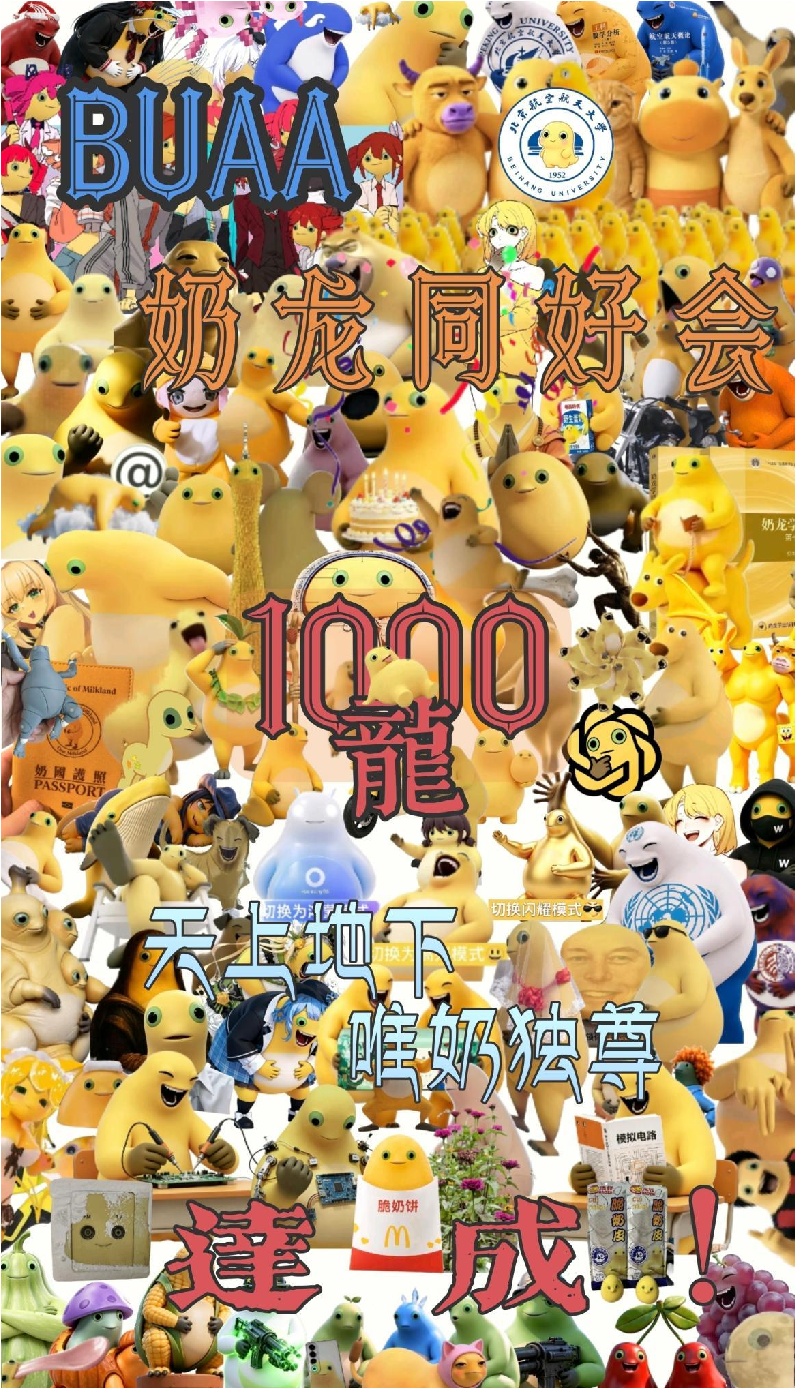
\includegraphics[width=324.7bp,height=0.90\textheight,keepaspectratio]{figures/chapter09/buaaPlate.pdf}
  \caption*{2026 年 10 月 12 日，北航奶龙同好会正式突破 1000 龙}
\end{figure}

\clearpage


